% 第二、三问附录；保留既有实验来源及负例轨迹。
\section*{附录A\quad 实验来源与复核口径}\label{sec:appendix-evidence}
\addcontentsline{toc}{section}{附录A 实验来源与复核口径}

各批次的代码、权重身份与来源SHA256见辅助材料 结构化实验证据索引。
下表仅用于定位证据，原始研究目录保留完整动作记录；
本轮论文整理未重新运行策略或训练模型。

\Needspace{38mm}
\begin{center}
\begin{minipage}{\linewidth}
\centering\small
\captionof{table}{已有实验的来源和用途}
\label{tab:q23-evidence}
\vspace{4pt}
\begin{tabular}{@{}lll@{}}
\toprule
证据 & 实验批次与样本 & 用途与边界 \\
\midrule
E01至E03 & 首版256随机与28压力 & 四方法完整方案对比，分布分开 \\
E04 & 每方法32局串行计时 & 已用开发场景上的计算开销 \\
E05、E06 & 各64局冻结后确认 & 上限静默、覆盖移站单组件增益 \\
E07 & 新256随机及28压力 & 相对静默、16源上限及组合 \\
E08至E10 & 训练链及开发端点 & PPO预算、GAE与失败探索 \\
E11、E12 & 后期48开发场景 & RL配对结果与原点全扫诊断 \\
E13 & 既有50局官方演练 & 冻结组合版的接口与执行验证 \\
\bottomrule
\end{tabular}
\end{minipage}
\end{center}

图\ref{fig:q23-1}、图\ref{fig:q23-2}为解析或算法示意；
图\ref{fig:q23-3}至图\ref{fig:q23-8}来源于既有数值记录。
图\ref{fig:q23-6}按基线中位耗时选取，图\ref{fig:q23-7}和图\ref{fig:q23-8}为事后最大退化例，不混入新增独立测试结论。
上述随机评估沿用其原始冻结与数据分割记录；
不将已经用于开发的场景重新称为未见测试。

写作组织参考了官方公开的2018年国赛B217与A440两篇匿名展示论文，其出处与获奖展示依据保存在 \texttt{references/references.md}。
它们只作为表达范例，本题公式和成绩均以本项目实现及实验为依据。
绘图使用Matplotlib及Scientific Visualization skill，其版本、软件文献和导出清单见配套README与参考资料。

\clearpage
\section*{附录B\quad 退化案例的轨迹对照}\label{sec:appendix-trajectories}
\addcontentsline{toc}{section}{附录B 退化案例的轨迹对照}

图\ref{fig:q23-7}为状态搜索相对前瞻基线退化最大的首版随机场景。
图\ref{fig:q23-8}为PPO相对前瞻基线退化最大的场景。
两图均显示全部四方法，不因展示负例而省略其他方法结果。

\begin{figure}[!htbp]
\centering
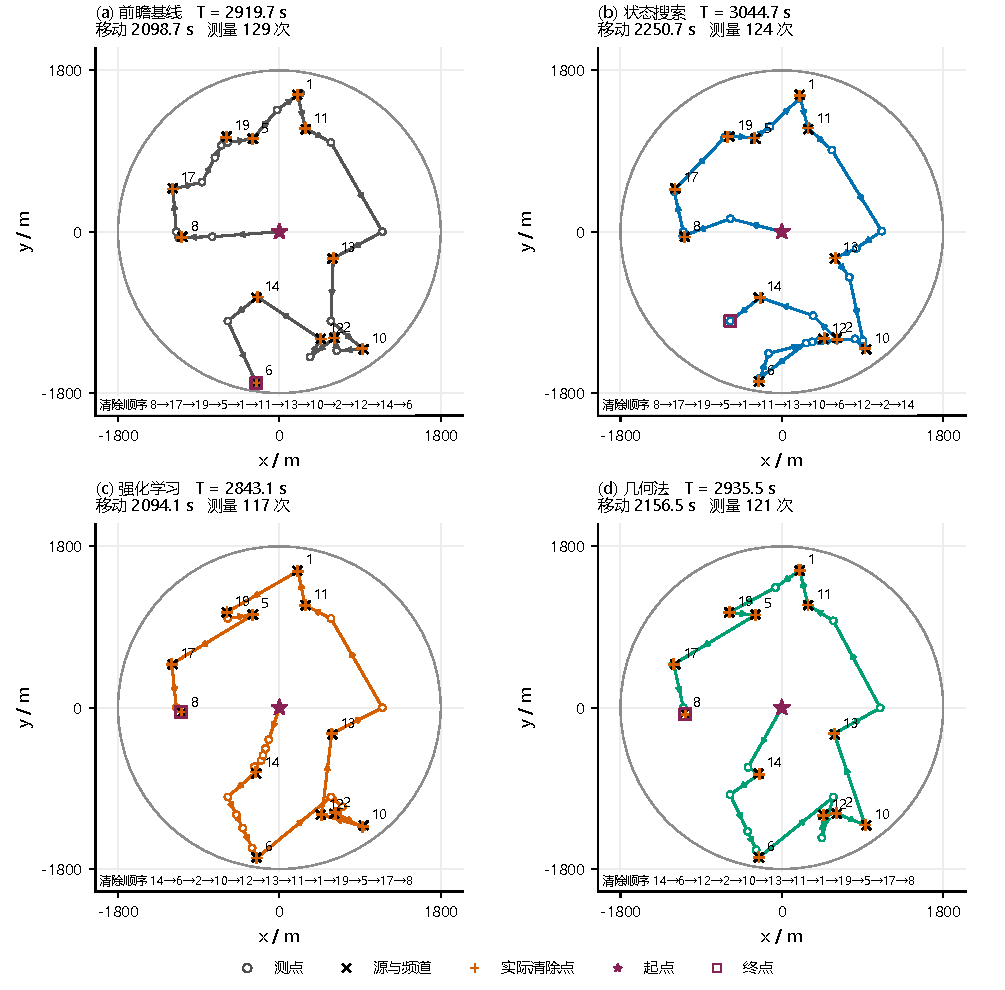
\includegraphics[width=\linewidth,height=\textheight,keepaspectratio,alt={状态搜索最大退化场景800015。状态搜索虽减少检测，却因移动增长而较基线慢125.08 s；此例为事后诊断选择。}]{figures/fig07_trajectory_state_worst.pdf}
\caption{状态搜索最大退化场景800015。状态搜索虽减少检测，却因移动增长而较基线慢125.08 s；此例为事后诊断选择。}
\label{fig:q23-7}
\end{figure}

\begin{figure}[!htbp]
\centering
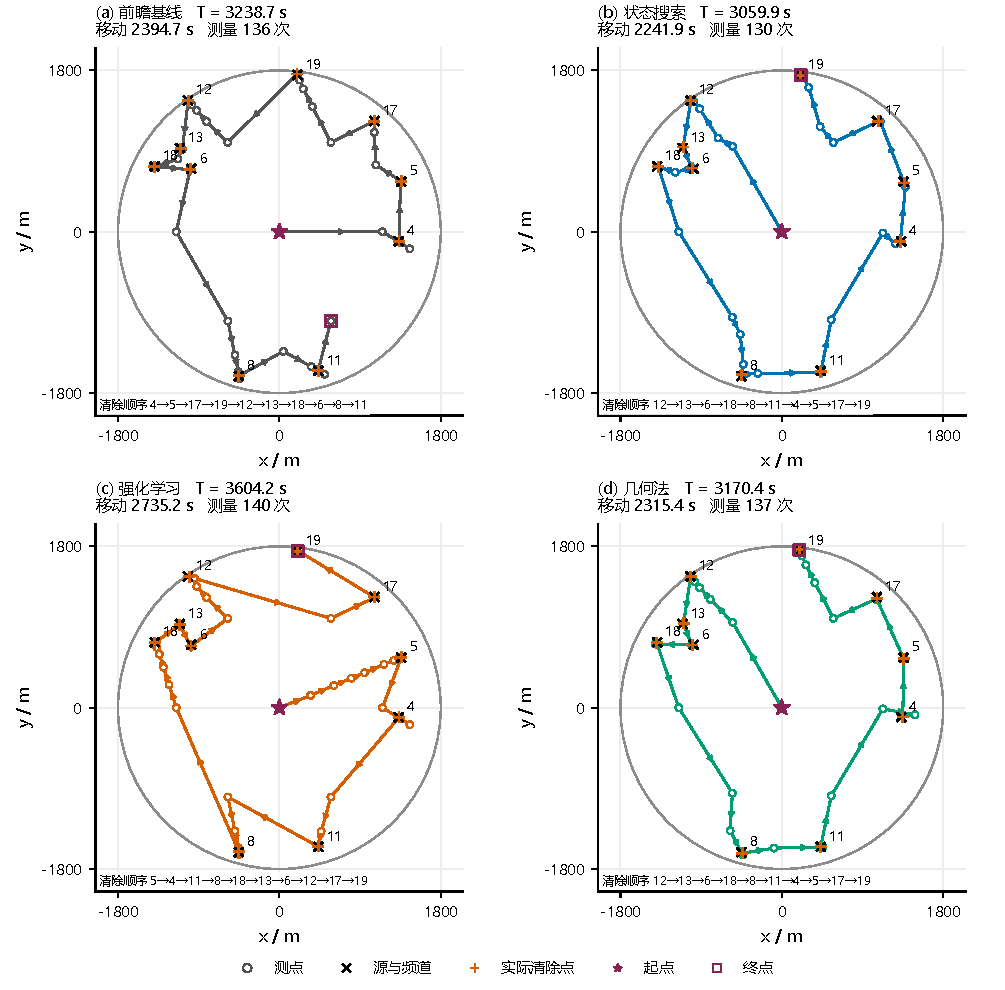
\includegraphics[width=\linewidth,height=\textheight,keepaspectratio,alt={PPO最大退化场景800081。该例主要额外代价来自移动，PPO较基线慢365.45 s；此例不表示总体发生频率。}]{figures/fig08_trajectory_rl_worst.pdf}
\caption{PPO最大退化场景800081。该例主要额外代价来自移动，PPO较基线慢365.45 s；此例不表示总体发生频率。}
\label{fig:q23-8}
\end{figure}

\FloatBarrier
